
\iffalse
\begin{figure}
    \centering
    \includegraphics[width=12cm]{../figures/blip_bbh_runs_two_panel_comparison.pdf}
    \caption{Glitch panel comparison}
    \label{fig:qscan_null}
\end{figure}
\fi

\section{Problem of glitches in the 3G-era}

\section{Introducing \texttt{nijntje} algorithm}
\subsection{The null stream of the Einstein Telescope}
\subsection{Toy model}
\subsection{Absence of null stream: ET-2L comparison}
\section{Precision science measurement with speed}
\section{Caveats}
\begin{figure}
    \centering
    \includegraphics[width=10cm]{../figures/et2l_delta_glitch_overlap_glitch_master.pdf}
    \caption{Glitch overlap}
    \label{fig:glitch_overlap}
\end{figure}

\begin{figure}
    \centering
    \includegraphics[width=10cm]{../figures/newsnr_mismatch_comparison.pdf}
    \caption{Mismatch}
    \label{fig:mismatch}
\end{figure}

\begin{figure}
    \centering
    \includegraphics[width=16cm]{../figures/newsnr_fig_4.pdf}
    \caption{Mass Distance Sky}
    \label{fig:delta_zero}
\end{figure}

\begin{figure}
    \centering
    \includegraphics[width=10cm]{../figures/newsnr_rank_10_single_block_percentile_parameters_short.pdf}
    \caption{Confidence interval}
    \label{fig:trend_delta}
\end{figure}

\begin{figure}
    \centering
    \includegraphics[width=16cm]{../figures/assemble_nijntje.pdf}
    \caption{The blue box outlines the workflow of \texttt{nijntje} algorithm. \textit{Step 1}: Construct the null stream by summing the strain data from three interferometers. \textit{Step 2}: Using the null stream data and an RJMCMC method, perform an unmodelled reconstruction of the glitch timeseries. \textit{Step 3}: Find the glitch timeseries which corresponds to the median of the posterior samples and subtract it from $\mathrm{ET}_1$ frame. \textit{Step 4} (Optional): Perform parameter estimation using the cleaned data from $\mathrm{ET}_1$, and the existing data from $\mathrm{ET}_2$ and $\mathrm{ET}_3$ to verify the accuracy.}
    \label{fig:nijntje_chart}
\end{figure}

